\section{Umsetzung}

\subsection{Datenbasis}

Als Grundlage dieser Arbeit wurde ein Korpus aus Texten von insgesamt 7 deutschsprachigen, der verschwörungstheoretiker Szene zuzurechnenden Internetangeboten erstellt.
Die Skripte zum automatischen Abruf der Texte nutzen das R-Paket \textit{rvest} \parencite{rvest} und extrahieren mittels für jede Seite separat erstellten CSS-Selektoren und XPATH-Queries den jeweiligen Artikeltext.
Während dieses Prozesses wurden auch kleinere Bereinigungen an den Texten vorgenommen, um wiederkehrende, nicht zum Artikeltext gehörende Elemente wie Werbung oder Spendenaufrufe zu entfernen, die Texte selbst wurden jedoch soweit möglich nicht weiter bearbeitet.
Weiterhin erfasst wurde zu jedem Artikel das (angegebene) Veröffentlichungsdatum, der Artikeltitel sowie die Rubrik auf der Website, so diese Angabe vorhanden war.

\begin{figure}[h]
    \centering
    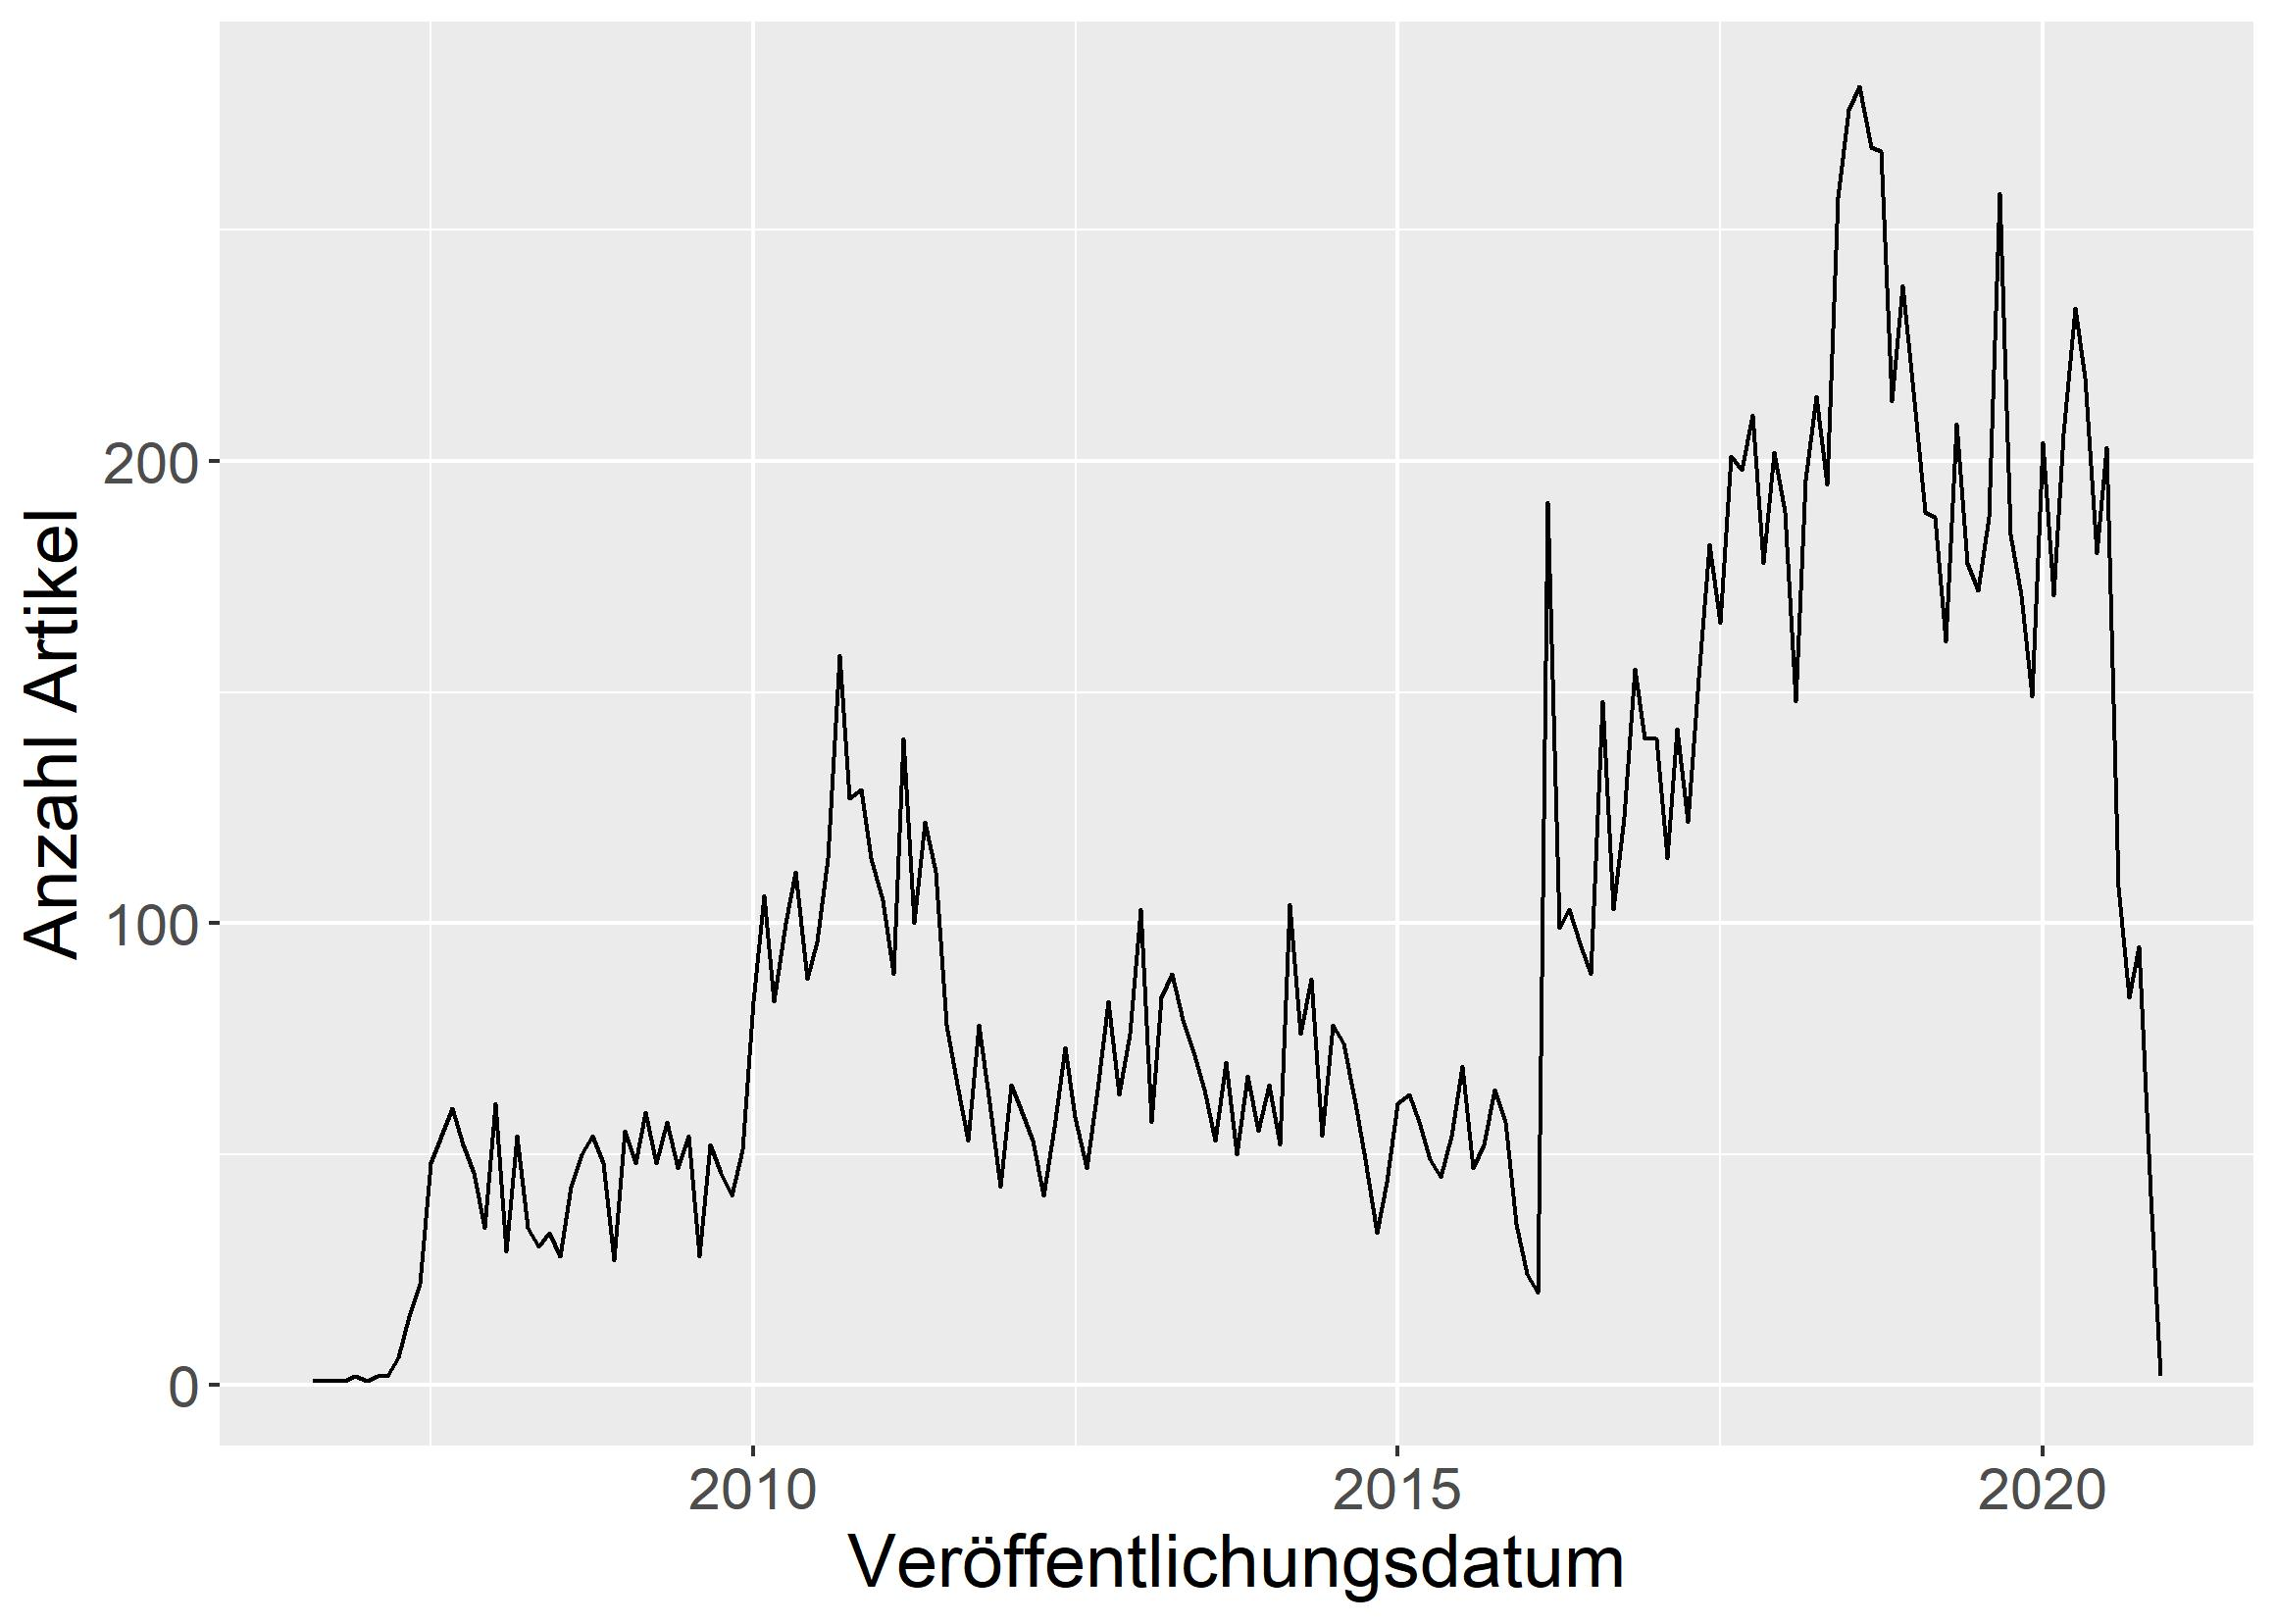
\includegraphics[scale=0.45]{graphics/cons_freq_time.jpg}
    \caption{Anzahl Artikel nach Veröffentlichungsdatum (nach Monat gruppiert)}
    \label{article-frequency}
\end{figure}

Der so erstellte Korpus umfasst insgesamt 16836 Texte und deckt beginnend in 2006 einen Zeitraum von 14 Jahren ab.
Die zeitliche Verteilung der Artikel im Korpus ist Grafik \ref{article-frequency} zu entnehmen, wie dort ersichtlich ist steigt beginnend in 2016 die Zahl der Artikel deutlich an.
Dies ist zum einen damit zu erklären, dass einzelne der gecrawlten Websites ihre Veröffentlichungsfrequenz zu dieser Zeit erhöht haben, überwiegend ist diese Entwicklung aber darauf zurückzuführen, dass insbesondere das Angebote von \textit{Watergate.tv} erst im Jahr 2016 seinen Betrieb aufgenommen hat und eine hohe Veröffentlichungsfrequenz aufweist. 
Genauere Informationen zu den von den einzelnen Angeboten abgedeckten Zeiträumen sowie zu Artikelzahl und Länge finden sich in Tabelle \ref{corpus-stats}.

Ebenso ist dort ersichtlich, dass sich nicht nur die absolute Zahl der Artikel nach Quelle stark unterscheidet, auch das Veröffentlichungsinterval schwankt je nach Quelle von weniger als einem Artikel/Monat zu über 100.
Es besteht weiterhin ein negativer Zusammenhang zwischen der Artikellänge und dem Veröffentlichungsintervall ($r = -0.72, p = 0.065$).

\begin{table}
    \begin{center}
        \begin{tabularx}{\textwidth}{l|XXXXX}
            \toprule
            & Von & Bis & Mittlere Zeichenzahl & Anzahl Artikel & Artikel/ Monat\\
            \midrule
            Alles Schall und Rauch & 23.08.06 & 02.08.20 & 5000 & 5349 & 32.0\\
            conrebbi & 05.09.12 & 20.10.14 & 5610 & 24 & 1.0\\
            deutschlandpranger & 29.10.16 & 30.12.20 & 7527 & 118 & 2.4\\
            fm-tv & 31.07.08 & 02.11.18 & 9158 & 97 & 0.8\\
            hinterderfichte & 16.01.10 & 31.05.18 & 4221 & 1083 & 10.8\\
            recentr & 03.08.07 & 05.08.20 & 5071 & 4762 & 30.5\\
            Watergate.tv & 20.05.16 & 16.11.20 & 2810 & 5403 & 101.9\\
            \bottomrule
            \end{tabularx}
        \caption{Kennzahlen der einzelnen Quellen des Korpuses}
        \label{corpus-stats}
    \end{center}
\end{table}

Auch eine inhaltliche Betrachtung zeigt deutliche Unterschiede zwischen den einzelnen Quellen.
So ist \textit{Alles Schall und Rauch} (\textit{ASuR}) als ältestes vertretenes Angebot auch einer der "klassischsten" Vertreter der Verschwörungswebsites.
Hier werden die Besucher:innen direkt auf der Startseite mit Fragen konfrontiert wie \enquote*{Was geschau wirklich am 11. September?} oder \enquote*{Was passiert tatsächlich mit dem Klima?} \parencite{asur-homepage}.
Hier lässt sich bereits die von \textcite[][205]{filatkina_2018} beobachtete Konstruktion des offenen Fragen finden, die die Aufmerksamkeit der Leser:innen auf sich ziehen soll.

Die Seite bedient sich klassischer Verschwörungstheorien und wird im allgemeinen der Truther Szene zugeordnet \parencite{psiram-asur}.
Sie hat laut Eigenaussage im Schnitt über 50.000 Zugriffe täglich.\footnote{Der Besucherzähler der Website ist inzwischen nicht mehr funktional, Angabe übernommen aus \textcite{vice-asur}}

Inhaltlich finden sich sowohl Essay-artige Artikel zu Themen wie 9/11, den Bilderberger-Treffen oder dem Klimawandel auf der Seite, aber auch kürzer gehaltene Meldungen zu aktuellen Ereignissen.
Es werden, wie bei fast allen anderen Seiten im Korpus, häufig Inhalte Dritter eingebunden sowie die Artikel durch Bilder oder Grafiken ergänzt.
Hier lässt sich Bereits die von \textcite{soukup_2008} beobachtete Multimedialität von Verschwörungstheorien beobachten.

Ähnlich zu \textit{ASuR} gelagert sind auch die Websites \textit{Hinter der Fichte} (\textit{HdF}) und \textit{conrebbi}, beide können der Truther Szene zugerechnet werden \cite[siehe etwa][]{psiram-conrebbi}.
In beiden Angeboten werden aktuelle Ereignisse kommentiert und verschwörungstheoretisch interpretiert, aber auch längere Essays zu typischen Themen der Szene verfasst.
Im Vergleich zu \textit{ASuR} werden bei beiden Angeboten deutlich mehr Inhalte in Form von Videos und Fremdquellen in Bild und Textform genutzt.

Von den bisherigen Quellen abheben tun sich dagegen die Angebote \textit{fm-tv} sowie \textit{Deutschlandpranger}.
Während sich beim \textit{Deutschlandpranger} etwa inhaltlich recht klassische Themen wie die Leugnung des Klimawandels \parencite*[vgl.][]{dprang-klima} finden, sind die dazugehörigen Text überdurchschnittlich lang und voller Werbung für Bücher zu z.T. komplett unabhängigen Themen.
Insbesondere aber sind die Texte selbst z.T. sehr wirr, die (sehr ausführlichen) AGB der Website enthalten etwa einen Abschnitt zu Strafzahlungen bei "Übersenden eines Statements anstatt einer echten Rechnung (True Bill) des wahren Haftungsgläubigers" \parencite*{dprang-agb} und weitere ähnlich obskure Paragraphen .

Die verbleibenden beiden Quellen im Korpus \textit{recentr} und \textit{Watergate.tv} sind beide der rechten truther Szene zuzuordnen und verbreiten Verschwörungstheorien in diese Richtung.
Beide zeichnet ein eher journalistischer Stil aus, es werden kurze bis mittellange Meldungen veröffentlicht, häufig begleitet von eigenen oder fremden Videos.
\textit{Recentr} wurde 2006 als deutscher Ableger von \textit{Inforwars.com} gegründet und bedient sich noch heute einem ähnlichen Konzept.
Ähnlich dem Vorbild wird massiv Werbung für den eigenen Shop gemacht in dem diverse Produkte zur Vorbereitung auf apokalyptische Szenarien sowie fragwürdige Nahrungsergänzungsmittel verkauft werden.
Inhaltlich sticht vor allem heraus, dass sich die Seite (bzw. der Hauptautor Alexander Benesch) z.T. sehr explizit von anderen Teilen der rechten/verschwörungstheoretischen Szene abgrenzt.
\footnote{So grenzt sich das Portal in Beiträgen inzwischen auch von \textit{Inforwars} Gründer Alex Jones ab \parencite*{recentr-jones} oder spekuliert darüber, ob die Alternative für Deutschland vom britischen Geheimdienst gegründet wurde \parencite{recentr-afd}}
So kommt es durchaus vor, dass in einem Artikel zunächst von der "implausiblen Sichtweise, verschiedenste Regierungen hätten eine Fake-Pandemie orchestriert" \parencite{recentr-population} gesprochen wird, nur um im nächsten Satz zu erklären: 

\begin{quotation}
    In Wirklichkeit sind die Methoden der globalen Bevölkerungsreduktion fast ausschließlich legal, simpel und werden schrittweise angewandt [...]. Das Konzept ist so entworfen, um mit möglichst wenig Zwang auszukommen [...]. \parencite{recentr-population}
\end{quotation} 

Die Website \textit{Watergate.tv} (inzwischen Teil von \textit{NEOPresse.com}) ist ein Nachrichten und Videoportal, das sich verschwörungstheoretischer Narrative bedient. 
Auf dem Portal finden sich klassische Themen wie Bilderberger-Treffen \parencite[vgl.][]{watergate-bilderberger} aber auch Fake-News und Berichterstattung mit starker pro-russischen Tendenz.
In die öffentlichkeit rückte das Portal als sich das Neo-Magazin-Royale wegen seiner Mitarbeit bei \textit{Watergate.tv} von Hans Meiser trennte \parencite*[Siehe z.B.][]{spiegel-watergate}.

Insgesamt deckt der hier verwendete Korpus einen signifikaten Teil der eher klassischen deutschsprachigen Truther Szene ab.
Es muss allerdings angemerkt werden, dass insbesondere in den letzten Jahren eine Bewegung in der Szene Richtung Social Media zu Portalen wie Facebook und Telegram stattfand.\todo{Eventuell noch ne Zitation reinwamsen.}
Diese zu Untersuchen ist allerdings nicht Teil der Fragestellung dieser Arbeit.

\subsection{Vergleichskorpus}

Um einen möglichst guten Vergleich zwischen den Texten im Korpus und dem Vergleichskorpus zu ermöglichen war es das Ziel Medien zu finden die in Form und inhaltlicher Ausrichtung dem Korpus möglichst ähnlich sind, ohne aber deren verschwörungstheretische Aspekte zu teilen.
Da insbesondere die letzten beiden besprochenen Angebote sich inhaltlich sehr an journalisitsche Angebote anlehnen, lag es nah ebensolche heranzuziehen.
Aus Gründen der Vollständigkeit (die Angebote sollten möglichst den kompletten Zeitraum des Korpus abdecken) sowie der Zugänglichkeit wurden die Angebote von \textit{Spiegel Online} sowie der \textit{Frankfurter Rundschau} ausgewählt.
Es wurde für beide Onlineangebote zunächst ein Index aller Artikel die in den selben Zeitraum wie der Korpus fallen erstellt und aus diesem zufällig eine Auswahl von 10000 Artikeln pro Anbieter gezogen.

Da die restlichen im Korpus enthaltenen Seiten alle mehr oder weniger in der Form eines Blogs gestaltet sind, sollten Angebote vergleichbarer Form herangezogen werden.
Um auch dem in der Literatur häufig genannten wissenschaftlichen Stil von verschwörungstheoretischen Texten Rechnung zu tragen wurde eine Reihe von Wissenschaftsblogs als zweite Komponente im Vergleichskorpus gewählt.
Dafür wurden von den beiden Platformen \textit{scienceblogs} und \textit{scilogs}\footnote{Beide Platformen sind Anbieter bei denen eine Vielzahl verschiedener Blogs zu finden sind.} ähnlich den journalistischen Angeboten aus dem gesamten Index der Einträge eine Auswahl von jeweils 10000 Artikeln ausgewählt.
Genauere Kennwerte zum Vergleichskorpus sind Tabelle \ref{comcorpus-stats} zu entnehmen.

\begin{table}
    \begin{center}
        \begin{tabularx}{\textwidth}{l|XXXXX}
            \toprule
            & Von & Bis & Mittlere Zeichenzahl & Anzahl Artikel & Artikel/ Monat\\
            \midrule
            Frankfurter Rundschau & 03.08.06 & 04.08.20 & 3670 & 9959 & 59.3\\
            scienceblogs & 14.02.07 & 04.08.20 & 3261 & 8765 & 54.4\\
            scilogs & 29.12.00 & 03.08.20 & 5206 & 9533 & 40.6\\
            Spiegel Online & 01.08.06 & 07.01.20 & 4687 & 8665 & 53.8\\
            \bottomrule
        \end{tabularx}
        \caption{Kennzahlen der einzelnen Quellen des Vergleiskorpuses}
        \label{comcorpus-stats}
    \end{center}
\end{table}

\subsection{Datenvorverarbeitung}

Zunächst wurden einige Süberungsverfahren auf den Korpus angewendet, um zu verhindern, dass fehlerhafte oder irrelevante Daten mit für die Feature Erstellung herangezogen werden.

Es wurde zunächst Unicode Normalisierung für alle Texte durchgeführt, anschließend wurde mittels des \textit{Google Compact Language Detector 3} \parencite[][]{cld3} die Sprache aller Text bestimmt und alle überwiegend Fremdsprachigen Artikel wurden aus dem Korpus entfernt.
Da im Korpus an einigen Stellen nicht zum Artikeltext gehörige Komponenten aus vielen Sonderzeichen vorhanden waren, wurden alle Wörter entfernt, die nur aus Zeichen bestanden, die unter 1000 Mal im gesamten Korpus vorhanden waren.
Weiterhin wurden noch kleinere Korrekturen vorgenommen, wie das Zusammenfassen multipler, aufeinanderfolgender Leerzeichen und Unterstriche (die gerne als Trennlinien in den Text benutzt wurden).

Abschließend wurden noch alle Text unter 100 Zeichen Länge aus dem Korpus entfernt, da diese für die Klassifizierungsaufgabe nur wenig Informationen enthalten können. Der finale Korpus umfasste 53758 Texte, mit einem Anteil der positiven Klasse (sprich von verschwörungstheoretischen Texten) von etwa 32\%.

\subsection{Features}

Zunächst wurden Features basierend auf den in der Literatur beobachteten linguistischen Eigenschaften von verschwörungstheoretischen Texten erstellt.
Die etwa von \textcite*[10]{miller_2002} festgestellte Emotionalität wird mit der Methode der Sentimentanalyse bearbeitet.
Dafür wurde das Sentimentwörterbuch \textit{SentiWS} \parencite[][]{sentiws} genutzt.
Dieses umfasst positive und negative Sentimentwerte für über 3000 Grundformen deutscher Wörter.
Während komplexere Ansätze wie etwa der von \textcite[]{ml_sentiment} eine höhere Präzision versprechen,\footnote{So ist der hier vorgestellte Ansatz nicht in der Lage korrekt mit Negationen umzugehen.} scheint die genutzte Methode für den vorliegenden Kontext ausreichende Ergebnisse zu lieferen.
Es wurde sowohl die Summe der positiven und negativen Sentimente erfasst, also auch die Summe sowie der Betrag nach Text insgesamt.
Hiermit soll insbesondere auf solche Fälle eingegangen werden, in denen ein Text zwar viele emotional behaftete Wörter verwendet, sich die Sentimentsumme aber durch einen Wechsel an positiven und negativen Wörtern ausgleicht.

Als weiteres in der Literatur anzutreffendes Merkmal soll auch die Menge an Zitationen betrachtet werden.
Um diese zu operationalisieren wurden zum einen die Anzahl der Anführungszeichen im Text gezählt.
Eine genauere Betrachtung der Verwendung von Fremdbelegen von denen etwa \textcite[235]{schafer_2018} spricht, wird ermöglicht indem als zusäztliche Features erfasst werden:
\begin{enumerate}
    \item Die Zahl der äußersten Zitate\footnote{Also Zitate die nicht Teil anderer Zitate sind}
    \item Die durchschnittliche Länge der Zitate
    \item Der Anteil von zitiertem Text am gesamten Artikeltext
\end{enumerate}

Die Menge an \textit{scare quotes} wird ebenfalls erfasst, wobei ein \textit{scare quote} für diese Arbeit definiert wird als ein Zitat in dem keine Leerzeichen (oder andere Formen von whitespaces) enthalten sind.

Die Menge der Fragen, wie sie etwa \textcite[205]{filatkina_2018} als Merkmal von verschwörungstheoretischen Texten feststellt, wird durch ein simples Zählen der im Text vorkommenen Fragezeichen abgebildet.
Ähnlich lässt sich auch die Annahme über die Häufung von Zahlenangaben wie sie sich bei \textcite[234]{schafer_2018} findet, durch einfaches Zählen von Zahlengruppen operationalisieren.
Um die bei \textcite[149]{stumpf_2019} gemachte Beobachtung der häufigen Verwendung von Negationswörtern abzubilden, wurde händisch eine Liste von 15 Negationswörtern erstellt und deren Häufigkeit in den Texten gemessen.

Die Multimedialität und Verknüpftheit von Verschwörungstheoretischen Online Texten wie sie \textcite[10]{soukup_2008} anspricht soll mit einer Reihe von Informationen die aus den dem Korpus zugrunde liegenden HTML Dateien extrahiert wurden abgebildet werden.
Um die Multimedialität zu erfassen wurde die Anzahl der eingebundenen Bilder, Tweets, Youtube-Videos sowie sonstiger eingebetteter Elemente im Artikel gezählt.
Für eine Messung der Verknüpftheit wurde die Anzahl von in den Artikeln enthaltenen Links, aufgeteilt nach internen und externen Zielen, erfasst.
Ebenso wurde als stilistisches Merkmal die Menge an fettgedruckten und kursiven Text erfasst.

\begin{table}
    \begin{center}
        \begin{tabularx}{\textwidth}{l|XXXXXX}
            \toprule
            Feature & \multicolumn{2}{X}{Korpus} & \multicolumn{2}{X}{Vergleichskorpus} & W & p\\
            & $\overline{X}$ & $\sigma$ & $\overline{X}$ & $\sigma$ & & \\
          \midrule
          Textlänge & 4309 & 4429 & 4208 & 4186 & \num{3.01e8} & $<0.01$\\
          Tweets & 0.0006 & 0.0058 & 0.0004 & 0.013 & \num{3.13e8} & $<0.01$\\
          Youtube-Videos & 0.016 & 0.088 & 0.004 & 0.037 & \num{3.45e8} & $<0.01$\\
          Interne Links & 0.0094 & 0.066 & 0.077 & 0.274 & \num{2.31e8} & $<0.01$\\
          Externe Links & 0.081 & 0.2 & 0.12 & 0.434 & \num{3.16e8} & $<0.01$\\
          Negationen & 0.158 & 0.11 & 0.151 & 0.109 & \num{3.23e8} & $<0.01$\\
          Anteil Zitation & 9.351 & 18.062 & 7.373 & 13.984 & \num{2.91e8} & $<0.01$\\
          Sentimente Betrag & 8.778 & 9.615 & 7.649 & 8.039 & \num{3.15e8} & $<0.01$\\
          \bottomrule
        \end{tabularx}
        \caption{Statistische Kennzahlen zu ausgewählten Features}
        \label{feature-stats}
    \end{center}
\end{table}

Um weitere Features aus dem Bereich der Textklassifikation zu nutzen, wurde der Corpus zunächst mithilfe von \textit{spaCy} \parencite[][]{spacy} annotiert um Lemmata und Part-of-Speech Tags zu generieren.
Es wurden anschließend die Anzahl jedes Part-of-Speech Tags sowie der Anteil an großgeschriebenen Text und Sonderzeichen als Feature übernommen.
Ebenso wurde die Wortdichte für jeden Text bestimmt, also die Anzahl an Wörtern im Verhältnis zur Textlänge.

Zur Ermittlung von Wortfrequenzen wurden zunächst Stopwörter aus dem Corpus entfernt\footnote{Zum Einsatz kam die Stopwort Liste aus dem \textit{tm} Paket \parencite[][]{r-tm}}, Wörter auf ihre Lemmata reduziert, einige Sonderfälle aussortiert\footnote{So wurde beispielsweise das Wort dpa nicht übernommen, da es praktisch exklusiv in Artikeln der Frankfurter Rundschau und von Spiegel Online vorkommt.} und anschließend die 400 häufigsten Wörter als Features übernommen.\footnote{Es ist durchaus üblich mehr Wörter als Features zu übernehmen \parencite*[siehe etwa][68]{feldman_sanger_2006}, da dies aber die Dimensionalität der Daten und damit die Komplexität der Klassifizierung deutlich erhöhen würde und die Auswahl von 400 Wörtern bereits zufriedenstellende Ergebnisse liefert wurde hier darauf verzichtet.}
Alle Features abgesehen von den sowieso als \textit{tf-idf} oder als relative Häufigkeit vorliegenden wurden mit der Textlänge skaliert.

\subsection{Modelerstellung}

Zunächst wurde ein Datensatz erstellt der alle Beobachtungen, aber nur solche Features enthielt die aus der Literatur zu Verschwörungstheorien abgeleitet wurden.
Auf diesem Datensatz wurde zunächst ein einfacher Entscheidungsbaum aus dem Paket \textit{rpart} \parencite[]{rpart} als Baseline Klassifizierer trainiert.
Hierfür wurde ein Train/Test Split im Verhältnis 2/1 auf den Daten durchgeführt.
Das auf den Trainingsdaten trainierte Modell erreichte eine Präzision von 75.3\%.


\begin{table}
    \begin{center}
        \begin{tabularx}{\textwidth}{X|XXXX}
            \toprule
            Modell & Accuracy & Sensitivity & Specificity & AUC\\
            \midrule
            dtree & 0.7534 & 0.7761 & 0.7428 & 0.829445 \\
            lightGBM & 0.8745 & 0.8700 & 0.8766 & .0.950817 \\
            \bottomrule
        \end{tabularx}
        \caption{Ergebnisse der Klassifizierer nur auf literaturbasierten Features}
        \label{small-model}
    \end{center}
\end{table}


Mit dem gleichen Daten wurde anschließend ein Modell mit der \textit{LightGBM} Bibliothek\parencite[][]{lightgbm} trainiert.
Da Gradienten-Boosting Verfahren schnell zu Overfitting neigen wurde dafür zunächst mittels Kreuzvalidierung auf den Trainingsdaten die optimale Iterationstiefe bestimmt.
Anschließend wurde das Modell mit einer Lernrate von 0.1 und einer maximalen Blattzahl von 50 trainiert.
Das so trainierte Modell erreichte eine Präzision von 87.4\%.

In Tabelle \ref{small-model} sind die Leistungen der beiden Modelle auf den Testdaten zusammengefasst.
Wie zu erkennen ist, ist selbst der einfache Entscheidungsbaum deutlich Präziser als es ein bloßes Raten im Klassenverhältnis wäre ($p < 0.01$).
Auch ist ersichtlich, dass das komplexere \textit{LightGBM} Modell eine in allen Bereichen deutlich bessere Klassifizierungsleistung erbringt.

\begin{table}
    \begin{center}
        \begin{tabularx}{\textwidth}{X|XXXX}
            \toprule
            Modell & Accuracy & Sensitivity & Specificity & AUC\\
            \midrule
            dtree & 0.8668 & 0.7845 & 0.9052 & 0.881973 \\
            lightGBM\footnotemark & 0.9784 & 0.9770 & 0.9791 & N/A \\
            \bottomrule
        \end{tabularx}
        \caption{Ergebnisse der Klassifizierer auf dem vollständigen Datensatz}
        \label{full-model}
    \end{center}
\end{table}


Im weiteren wurde ein Modell mit allen vorhandenen Features erstellt.
Hierfür wurde ebenfalls zunächst ein Baseline Entscheidungsbaum trainiert.
Dieser erreichte eine Präzision von 87.7\% und konnte damit den Entscheidungsbaum der auf dem kleineren Korpus trainiert wurde in Genauigkeit deutlich übertreffen.
Interessant ist vor allem die verhältnismäßig geringe Sensitivität.

\begin{figure}[ht]
    \centering
    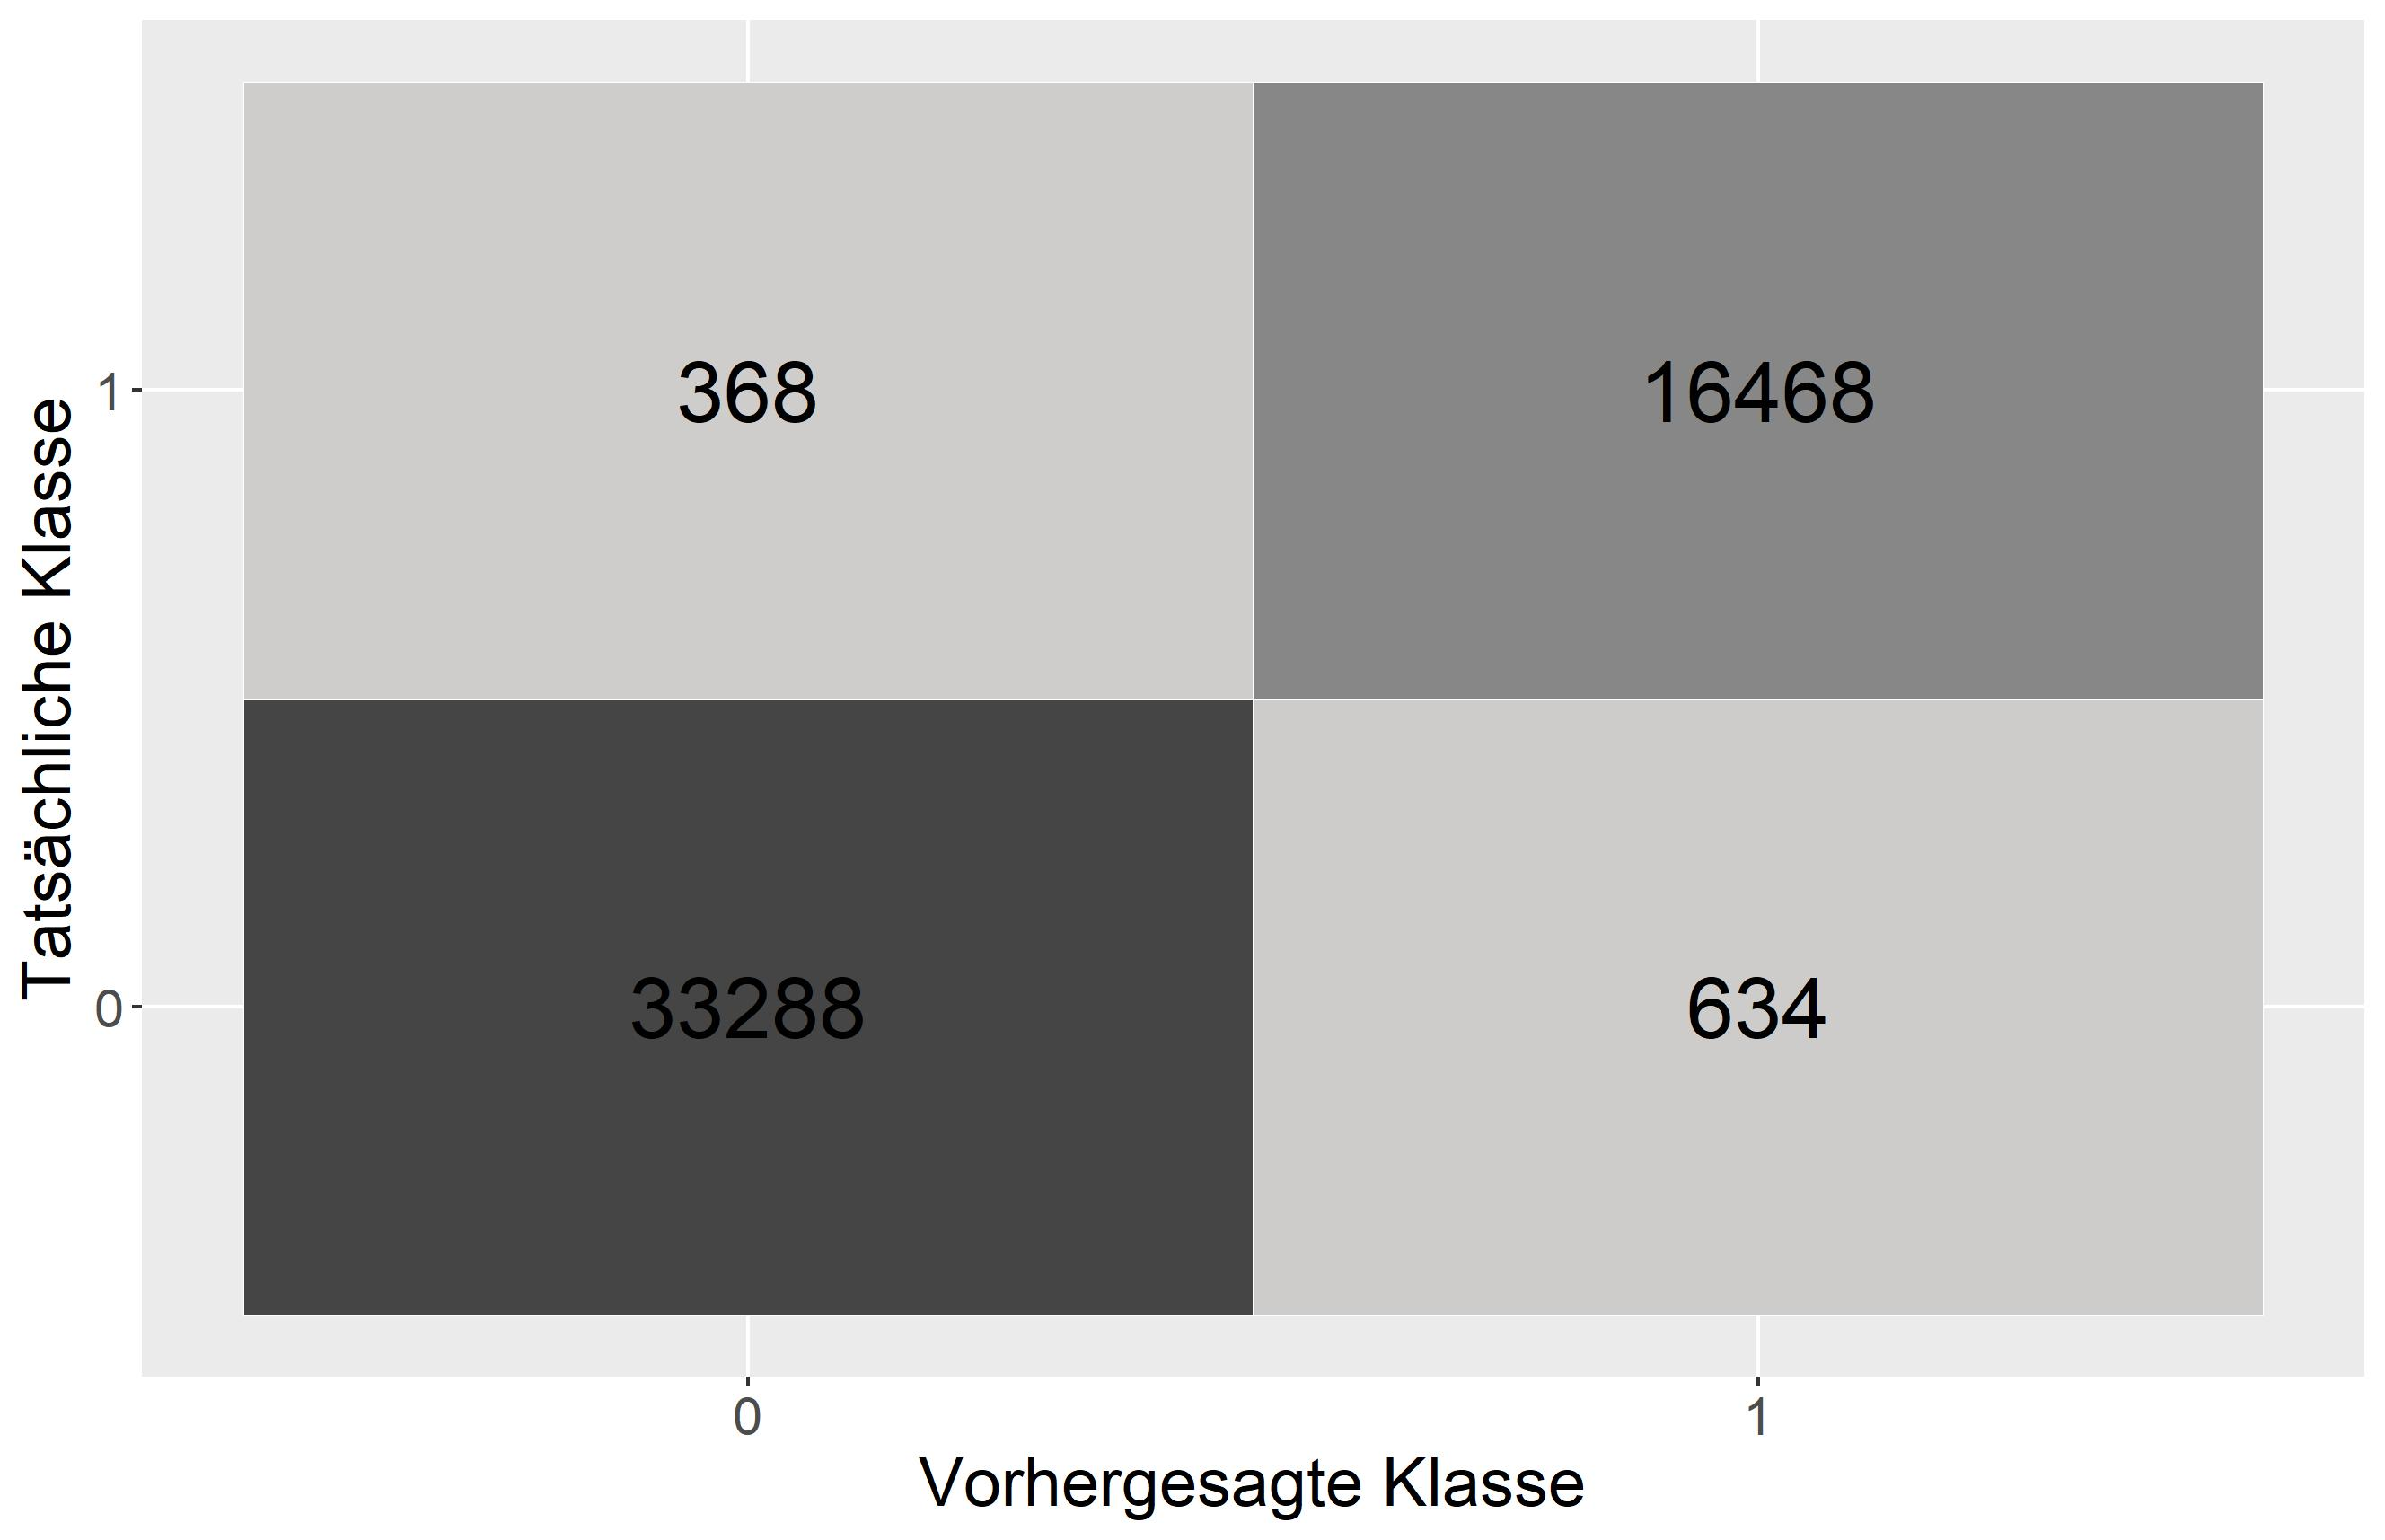
\includegraphics[scale=0.45]{graphics/confusion_matrix.jpg}
    \caption{Confusion-Matrix der 10-Fold Kreuzvalidierung des finalen Models}
    \label{confusion-table}
\end{figure}

% \begin{table}
%     \begin{center}
%         \begin{tabularx}{\textwidth}{XX|XX}
%             \cmidrule{3-4}
%             & & \multicolumn{2}{X}{Referenz}\\
%             & & 0 & 1 \\
%             \hline
%             \multirow{2}{*}{Vorhersage} & 0 & 33288 & 368 \\
%             \cmidrule{2-4}
%             & 1 & 634 & 16468 \\\midrule
%         \end{tabularx}
%         \caption{Confusion-Table des finalen Modells}
%         \label{confusion-table}
%     \end{center}
% \end{table}

Bevor das finale Modell trainiert wurde, wurde zunächst mittels eines Tunegrids eine optimierung der Hyperparameter der Lernrate sowie der Anzahl der äußersten Blätter durchgeführt.
Getestete Werte waren dabei für die Lernrate 0.01, 0.05, 0.10, 0.20 und für die Blätterzahl 5, 50, 127 (Der Standardwert von lightGBM), 200.
Das beste Ergebnis wurde mit einer Lernrate von 0.05 und einer Blätterzahl von 50 erzielt.
Mit diesen Werten wurde erneut die optimale Iterationstiefe mittels Kreuzvalidierung bestimmt.
Das mit diesen Parametern erstellte, finale Modell wurde schließlich mittels einer 10-Fold Kreuzvalidierung validiert und erreichte insgesamt eine Präzision von 98.14\%.

\footnotetext{10-Fold Kreuzvalidiert}
